%%%%%%%%%%%%%%%%%%%%%%% file template.tex %%%%%%%%%%%%%%%%%%%%%%%%%
%
% This is a general template file for the LaTeX package SVJour3
% for Springer journals.          Springer Heidelberg 2010/09/16
%
% Copy it to a new file with a new name and use it as the basis
% for your article. Delete % signs as needed.
%
% This template includes a few options for different layouts and
% content for various journals. Please consult a previous issue of
% your journal as needed.
%
%%%%%%%%%%%%%%%%%%%%%%%%%%%%%%%%%%%%%%%%%%%%%%%%%%%%%%%%%%%%%%%%%%%
%
% First comes an example EPS file -- just ignore it and
% proceed on the \documentclass line
% your LaTeX will extract the file if required
\begin{filecontents*}{example.eps}
%!PS-Adobe-3.0 EPSF-3.0
%%BoundingBox: 19 19 221 221
%%CreationDate: Mon Sep 29 1997
%%Creator: programmed by hand (JK)
%%EndComments
gsave
newpath
  20 20 moveto
  20 220 lineto
  220 220 lineto
  220 20 lineto
closepath
2 setlinewidth
gsave
  .4 setgray fill
grestore
stroke
grestore
\end{filecontents*}
%
\RequirePackage{fix-cm}
%
%\documentclass{svjour3}                     % onecolumn (standard format)
%\documentclass[smallcondensed]{svjour3}     % onecolumn (ditto)
%\documentclass[smallextended]{svjour3}       % onecolumn (second format)
\documentclass[twocolumn]{svjour3}          % twocolumn
%
\smartqed  % flush right qed marks, e.g. at end of proof
%
\usepackage{graphicx}
\usepackage{xspace}
\usepackage{hyperref}
%
% \usepackage{mathptmx}      % use Times fonts if available on your TeX system
%
\usepackage{url}
% insert here the call for the packages your document requires
%\usepackage{latexsym}
% etc.
%
% please place your own definitions here and don't use \def but
% \newcommand{}{}
\newcommand{\Openstack}{\texttt{Open\-Stack}\xspace}
\newcommand{\Roced}{\texttt{Roced}\xspace}
\newcommand{\ATLAS}{ATLAS\xspace}
\newcommand{\CMS}{CMS\xspace}
\newcommand{\NEMO}{NEMO\xspace}
\newcommand{\Packer}{\texttt{Packer}\xspace}
\newcommand{\Puppet}{\texttt{Puppet}\xspace}
\newcommand{\Hieradata}{\texttt{Hieradata}\xspace}
\newcommand{\Moab}{\texttt{Moab}\xspace}
\newcommand{\Slurm}{\texttt{Slurm}\xspace}
\newcommand{\BeeGFS}{\textsc{BeeGFS}\xspace}
\newcommand{\OZ}{\texttt{Oz}\xspace}
\newcommand{\HTCondor}{\texttt{HTCondor}\xspace}
\newcommand{\kickstart}{\texttt{kickstart}\xspace}
\newcommand{\sinfo}{\texttt{sinfo}\xspace}

\hyphenation{
phys-ics
re-search
start-ed
}


\usepackage{lineno}
\linenumbers

% Insert the name of "your journal" with
\journalname{Computing and Software for Big Science}
%
\begin{document}

\title{Dynamic Virtualized Deployment of Particle Physics Environments on a
  High Performance Computing Cluster%\thanks{Grants or other notes
%about the article that should go on the front page should be
%placed here. General acknowledgments should be placed at the end of the article.}
}
%\subtitle{Do you have a subtitle?\\ If so, write it here}

%\titlerunning{Short form of title}        % if too long for running head

%
%
\author{Felix B\"uhrer \and Frank Fischer \and Georg Fleig \and Anton
  Gamel \and Manuel Giffels \and Thomas Hauth \and Michael Janczyk
  \and Konrad Meier \and
G\"unter Quast \and  Beno\^it Roland \and
  Markus Schumacher \and Ulrike Schnoor \and Dirk von Suchodoletz \and Bernd Wiebelt
%  % etc.
}



%\authorrunning{Short form of author list} % if too long for running head

\institute{ F. B\"uhrer \at Universit\"at Freiburg, Physikalisches
  Institut, Hermann-Herder-Str. 3, 79104 Freiburg, Germany
  \and F. Fischer \at Karls\-ruher Institut f\"ur Technologie, Institut f\"ur Experimentelle
  Teilchenphysik, Wolfgang-Gaede-Str. 1, 76131 Karls\-ruhe, Germany
 \and G. Fleig \at Karls\-ruher Institut f\"ur Technologie, Institut f\"ur Experimentelle
Teilchenphysik, Wolfgang-Gaede-Str. 1, 76131 Karls\-ruhe, Germany
  \and A. Gamel  \at  Universit\"at Freiburg, Physikalisches
  Institut, Hermann-Herder-Str. 3, 79104 Freiburg, Germany \at  Universit\"at Freiburg, Rechenzentrum, Hermann-Herder-Str.10, 79104
  Freiburg, Germany
  \and M. Giffels \at Karls\-ruher Institut f\"ur Technologie, Institut f\"ur Experimentelle
  Teilchenphysik, Wolfgang-Gaede-Str. 1, 76131 Karls\-ruhe, Germany
  \and T. Hauth \at Karls\-ruher Institut f\"ur Technologie, Institut f\"ur Experimentelle
  Teilchenphysik, Wolfgang-Gaede-Str. 1, 76131 Karls\-ruhe, Germany
  \and M. Janczyk \at  Universit\"at Freiburg, Rechenzentrum,
  Hermann-Herder-Str. 10, 79104
  Freiburg, Germany
  \and K. Meier  \at  Universit\"at Freiburg, Rechenzentrum,
  Hermann-Herder-Str. 10, 79104
  Freiburg, Germany
  \and G. Quast \at Karls\-ruher Institut f\"ur Technologie, Institut f\"ur
  Experimentelle Teilchenphysik, Wolfgang-Gaede-Str. 1, 76131
  Karls\-ruhe, Germany
  \and  B. Roland \at  Universit\"at Freiburg, Physikalisches
  Institut, Hermann-Herder-Str. 3, 79104 Freiburg, Germany
  \and  M. Schumacher \at  Universit\"at Freiburg, Physikalisches
  Institut, Hermann-Herder-Str. 3, 79104 Freiburg, Germany
  \and  U. Schnoor \at   Universit\"at Freiburg, Physikalisches
  Institut, Hermann-Herder-Str. 3, 79104 Freiburg, Germany 
  \at \emph{Now at} CERN, CH-1211 Geneva
  23, Switzerland        %  \\
  \\\email{ulrike.schnoor@cern.ch}   
 \and D. von Suchodoletz \at Universit\"at Freiburg, Rechenzentrum,
 Hermann-Herder-Str. 10, 79104
  Freiburg, Germany 
 \and B. Wiebelt \at Universit\"at Freiburg, Rechenzentrum,
 Hermann-Herder-Str. 10, 79104
 Freiburg, Germany
}



\date{Received: date / Accepted: date}
% The correct dates will be entered by the editor


\maketitle

\begin{abstract}
The \NEMO High Performance Computing Cluster at the University of
Frei\-burg has been made available to
researchers of the \ATLAS and \CMS experiments.
Users access the cluster from external machines connected to the
World-wide LHC Computing Grid (WLCG).
 This paper describes how the full software environment of the WLCG
 is provided in a virtual machine image. The interplay between the
 schedulers for \NEMO and for the external
 clusters is coordinated through the \Roced service.
A cloud computing infrastructure is deployed at \NEMO to orchestrate the
simultaneous usage by bare metal and virtualized jobs.
Through the setup, resources are provided to users in a transparent,
automatized, and
on-demand way. The performance of the virtualized environment has been
evaluated for particle physics applications.

%Insert your abstract here. Include keywords, PACS and mathematical
%subject classification numbers as needed.
\keywords{Virtualization \and Particle Physics \and Grid Computing
  \and Benchmarks \and Opportunistic Usage}
% \PACS{PACS code1 \and PACS code2 \and more}
% \subclass{MSC code1 \and MSC code2 \and more}
\end{abstract}




\section{Introduction}
\label{intro}
This paper presents the concepts and implementation of providing a HPC resource
to ATLAS and CMS users accessing external clusters connected to the World-wide
computing grid (WLCG) with the purpose of running data production as well as
data analysis on the HPC host system.  For this purpose, the HPC cluster NEMO at
the University of Freiburg is deploying an OpenStack instance to handle the
virtual machines.  The schedulers on the NEMO and the external resources are
connected through the ROCED service\cite{ROCED}.

The CMS and ATLAS groups cooperated in this project with the HPC team of the
eScience group of the computer center of University of Freiburg (UFR) to tackle
the particular challenges of VREs like provisioning, setup, scheduling and
decommissioning. A VRE in the context of this paper is a complete software stack
as it would get installed on a compute cluster fitted to ATLAS or CMS groups
demand.



\section{Virtualization infrastructure}
\label{sec:openstack}

Motivation for virtualized approach (increase the number of potential
user groups without increasing the administrative effort); virtualized
research environments; description of infrastructure for virtualized research environments
(OpenStack, startVM etc) on NEMO 


\section{Generation of the VRE image}
The VREs for ATLAS and CMS software environments consist in \Openstack containers
in the format of compatible VM images.
These images are provided in an automatized
way allowing versioning and archiving of the environments captured in
the images.
% The approaches used in the
% different groups are described in the following.

\subsection{\Packer combined with \Puppet}


One approach to generating the image is the open-source tool
\texttt{packer}~\cite{packer}, interfaced to \texttt{puppet}~\cite{puppet}.
\texttt{Packer} allows to configure an image based on an \texttt{.iso} file using a kickstart~\cite{kickstart} file and flexible script-based configuration. 
It also provides an interface to \texttt{puppet} making it a convenient tool if an existing \texttt{puppet} role is to be used for the images. If the roles are defined according to the hostname of the machine as is conventional in \texttt{puppet} with \texttt{hieradata}, the hostname needs to be set in the scripts supplied to \texttt{packer}. Propagation of certificates require an initial manual start of a machine with the same hostname to allow handshake signing of the certificate from the \texttt{puppet} server.

Apart from these initial adjustments, \texttt{packer}'s interface to \texttt{puppet} allows a fully automated image generation with up-to-date configuration.




\subsection{Image generation using the \OZ toolkit}
%$\to$CMS Karlsruhe\\
Another option to employ a fully-automated procedure is to use the OZ toolkit~\cite{OZ}. All requirements and configuration options of an image can be specified via an XML file, called template. The partitioning and installation process of the operating system is fully automated, as OZ will use the remote-control capabilities of the local hypervisor. After the installation of the operating system, additional libraries and configuration files can be installed. Once the image has been built, it is automatically compressed and uploaded to a remote cloud site.
Using this technique allows to build images in a reproducible fashion, as all templated files are version controlled using git. Furthermore, existing template files are easy to adapt to new sites and experiment configurations.




\section{Interfacing batch systems and virtual resources using \Roced}
\label{section:roced}
While HPC systems with support for virtualized research environments and commercial cloud providers offer the
necessities to acquire computing and storage capacity by dynamic
resource booking, the computing needs of high energy physics
re\-search groups ad\-di\-tion\-al\-ly require work\-flow
ma\-na\-ge\-ment sys\-tems capable of maintaining thousands of batch
jobs. Some cloud providers, for example Amazon with AWS
Batch~\cite{awsbatch}, provide a service for workflow management,
however these offerings are often limited to one specific cloud instance. To dynamically distribute batch jobs to multiple sites and manage machine life-time on specific sites, a combination of a highly-scalabe batch system and a virtual machine scheduler is desirable.

\subsection{\Roced}
\begin{figure*}
\begin{center}
  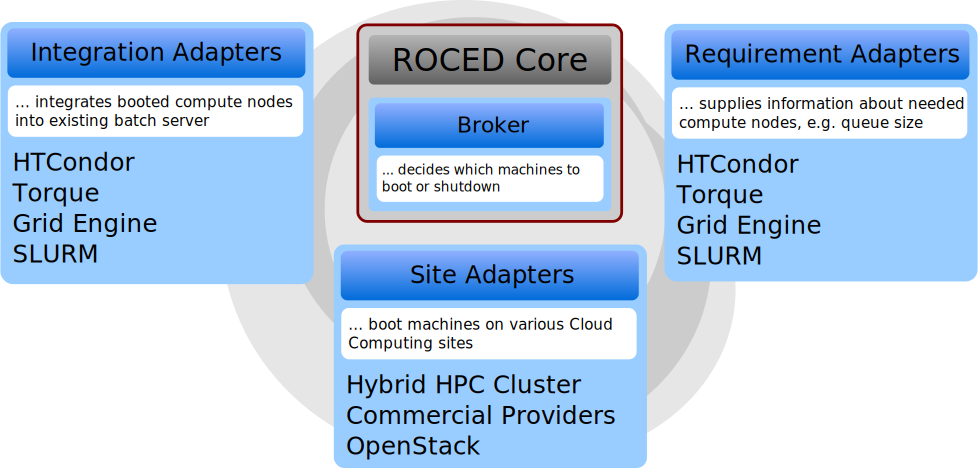
\includegraphics[width=0.9\linewidth]{figures/roced_design_flat.pdf}
  \caption{Overview of the \Roced modular design. The  \Roced Core contains the Broker which decides when and on which sites new virtual machines are booted. The Requirement Adapters report about the utilization and resource requirements of the attached batch systems. The Site Adapter is responsible to manage the lifetime of virtual machines on an cloud site and the Integration Adapter ensure that newly booted machines are integrated into the batch system.}
  \label{fig-roced}
\end{center}
\end{figure*}

%$\to$ CMS Karlsruhe
Many capable batch systems exist today and they can be interfaced to virtualization providers using the cloud meta-scheduler \Roced (Responsive On-demand Cloud Enabled Deployment) which has been developed at the KIT since 2010~\cite{ROCED}. \Roced is written in a modular
fashion in python and the interfaces to batch systems and cloud sites
are implemented as so-called \textit{Adapters}. This makes \Roced
independent of specific user groups or workflows. It provides a
scheduling core which collects the current requirement of computing
resources and decides if virtual machines need to be started or can be
stopped. One or more Requirement Adapters report the current queue
status of batch systems to the central scheduling core. Currently,
Requirement Adapters are implemented for the Slurm, Torque/Moab, HTCondor
and GridEngine batch systems. The Site Adapters allow \Roced to start,
stop, and monitor virtual machines on multiple cloud
sites. Implementations exist for Amazon EC2, OpenStack, OpenNebula and
Moab-based virtualization at HPC centers. Special care has been put
into the resilience of \Roced: it can automatically terminate
non-responsive machines and restart virtual machines in case some
machines have dropped out. This allows VM setups orchestrated by \Roced with thousands of virtual machines and many tens of thousands of jobs to run in production environments.
The modular design of \Roced is shown in Fig.~\ref{fig-roced}.

\subsection{Using \HTCondor as front-end scheduler}\label{sec:ROCED:HTCondor}
%$\to$ CMS Karlsruhe
The open-source HTCondor project provides a workload management system which is highly configurable and modular~\cite{HTCondor}. Batch processing workflows can be submitted and are then forwarded by HTCondor to idle resources. HTCondor maintains a resource pool, which worker nodes in a local or remote cluster can join. Once HTCondor has verified the authenticity and features of the newly joined machines, computing jobs are automatically transferred. Special features to connect from within isolated network zones, for example via a NAT-Portal, to the central HTCondor pool are available. The Connection Brokering (CCB) service is especially valuable to connect virtual machines to the central pool. These features and the well-known ability of HTCondor to scale to O(100k) of parallel batch jobs lets us decide to use HTCondor as a workload management system.

The virtual machines spawned for the CMS user group of the KIT come with the HTCondor client (\texttt{startd}) pre-installed and this client is started after the machine has fully booted and connects to the central HTCondor pool at the KIT via a shared secret. Due to HTCondor's dynamic design, new machines in the pool will automatically receive jobs and the transfer of the job configuration and meta-data files is handled via HTCondor's internal file transfer systems.

\subsection{Using \Slurm as front-end scheduler}
%$\to$ ATLAS Freiburg\\
Alternatively to the approach described above, the
open-source workload managing system \Slurm~\cite{Slurm} has been interfaced into \Roced by
the ATLAS group at University of Freiburg.
\Slurm provides a built-in functionality for the dynamic
startup of resources in the \textit{Slurm Elastic Computing}
module~\cite{SlurmElastic}.
However, this module has been found to be unsuitable for resources which are not
expected to be available within a fixed time period, in this case due to
the presence of a queue in the host system which may postpone the start
of a resource by a significant, varying period.
In addition the transfer of information, such as error states, from one scheduler to the
other, and therefore to the user, is very limited.
Therefore, \Roced has been chosen as the interface between the
\Moab scheduler on the host system and the \Slurm
scheduler on the submission side.


\begin{figure}

\includegraphics[width=0.95\linewidth]{figures/virtualisierung_ROCED.png}
\caption{Implementation of \Roced with \Slurm on the BFG cluster used by ATLAS researchers.}
\label{fig:slurmRocedBFG}
\end{figure}

The scheduling system is illustrated in Fig.~\ref{fig:slurmRocedBFG}.
For \Slurm, it is necessary that each potential virtual
machine is registered in the configuration at the time of start of the
\Slurm server as well as the client. \Slurm configurations also
need to be in agreement between server and client.
Therefore, a range of hostnames is registered in the configuration in
a way that is mapped to potential IP addresses of virtual machines.
These virtual machines have a fixed number of CPUs and memory assigned and are
registered under a certain \Slurm partition.
When a job is submitted to this partition and no other resource is
available, information from the \Slurm \texttt{squeue} and
\texttt{sinfo} commands is requested and parsed for the required information.

Since the ATLAS Freiburg group comprises three sub-groups, each mapped
to a different production account on \NEMO, special care is taken to
avoid interference of resources used by another account to ensure fair share on \NEMO, while
allowing jobs from one group to occupy otherwise idle resources of another group.

\Roced determines the amount of virtual machines to be started and sends the
corresponding VRE job submission commands to \Moab.
After the virtual machine has booted, the hostname is set to the IP
dependent name which is known to the \Slurm configuration.
A \texttt{cron} job executes several sanity
checks on the system.
Upon successful execution of these tests, the \Slurm client
running in the VM starts accepting the queued jobs.
After completion of the jobs and a certain period of receiving no new jobs from the queue, the
\Slurm client in the machine drains itself and the machine
shuts itself down.
The IP address as well as the corresponding hostname in \Slurm
are released and can be reused by future VREs.



\section{Analysis of performance and usage}

The ROCED-based solution described above has been implemented and put into production by the research groups at the University of Freiburg (Institute of Physics) and the Karlsruhe Institute of Technology (Institute of Experimental
Particle Physics). To prove the usefulness of this approach
statistical analyses of the performance of the virtualized setup both
in terms of CPU benchmarks and usage statistics have been conducted.

\subsection{Benchmarks}
%$\to$ ATLAS Freiburg\\
Besides the use of the legacy HEP-SPEC06 (HS06) benchmark \cite{Hepspec}, the performance of the compute resources is furthermore evaluated with two fast benchmarks
developed to provide real-time information of the WLCG performance and available in the CERN benchmark suite \cite{Alef:2017jyx}; the Dirac Benchmark 2012 DB12 \cite{DB12}
and the ATLAS Kit Validation KV \cite{DeSalvo:2010zza}. The DB12 program is evaluating the performance of CPUs through floating-point arithmetic operations, while the KV benchmark
is making use of the simulation toolkit GEANT4 \cite{Agostinelli:2002hh} to simulate the interactions of single muon events in the detector of the ATLAS experiment. As our primary
target is to measure performances of CPUs in the context of High Energy Physics applications, the KV benchmark constitutes a realistic workload. The DB12 benchmark is using
the HS06 units, and the KV output provides the number of events produced per second. \\

To assess the impact of the virtualisation, the performance of the same hardware configuration (20 cores Intel Xeon E5-2630 CPUs) has been determined either deployed via
the standard bare metal operation on the NEMO cluster (NEMO bare metal) and on the local ATLAS Tier-3 centre in Freiburg (ATLAS-BFG bare metal), or as virtual machines on the
NEMO cluster (NEMO VM). On the ATLAS-BFG bare metal and on the virtual machines running on the NEMO cluster, hyper-threading (HT) technology is activated. Both are using Scientific
Linux 6 \cite{SL6} as operating system. The NEMO bare metal has no HT activated due to the more general use case of the system, and uses CentOS7 as operating system \cite{CentOS7}. % \\
The scores of the HEP-SPEC06, DB12, and KV benchmarks have been determined for these three configurations as a function of the number of cores actually used by the benchmarking processes.
This number ranges from 2 to 40 for the ATLAS-BFG bare metal and for the NEMO VM, for which HT is enabled, and from 2 to 20 for the NEMO bare metal,
for which HT is not implemented. The results have been determined by step of two core units. The benchmarks have been run 20 times for each core multiplicity value, and the means
and standard deviations of the corresponding distributions have been extracted. \\

\begin{figure}[htbp]
\centering
\includegraphics[width=0.44\textwidth]{figures/benchmark-hepspec06-total.pdf}
\includegraphics[width=0.44\textwidth]{figures/DB12-BFG-BM-NEMO-VM-NEMO-BM-total.pdf} 
\includegraphics[width=0.44\textwidth]{figures/kv-BFG-BM-NEMO-VM-NEMO-BM-total.pdf} 
\caption{Total score as a function of the core multiplicity for the HEP-SPEC06 (top), DB12 (middle) and KV (bottom) benchmarks
for the ATLAS-BFG bare metal (blue open circles), the NEMO VMs (red full circles) and the NEMO bare metal (black open squares). The data points represent
the average values of the benchmarks for each core multiplicity, and the vertical bars show the associated standard deviations.}
\label{bmk-total}
\end{figure}

The total scores are presented in Fig.~\ref{bmk-total} for the three benchmarks and the three configurations considered, except for the KV software for which the NEMO bare metal
results are not yet available. The total scores observed for the different benchmarks are increasing until the maximum number of physical cores has been reached, and are characterized by a flattening increase
or a constant behaviour afterwards. The benchmark scores of the virtual machines running on the NEMO cluster are only slightly lower than those obtained for the NEMO bare metal operation, and the lost of performance
due to the virtualisation does not exceed 10$\%$. For the ATLAS-BFG bare metal and the VMs running on the NEMO cluster, the interplay between the virtualisation and the different operating systems leads
to similar benchmark behaviours for the two configurations.

% References for HEPSPEC
%%https://indico.cern.ch/event/49388/contributions/2014772/attachments/960838/1363966/20090127_NewCPUbenchmark_final.pdf
%%http://w3.hepix.org/benchmarking.html
%%https://spec.org/benchmarks.html
%%

%
%realistic load: as user
%machine reserved: root
%Hier sieht man, dass die Bare-Metal-User-Jobs wesentlich weniger performant sind, und die User-Jobs auf den VMs beinahe an die ROOT-Tests auf bare-metal herankommen. Interessant ist auch, dass bei den User-Jobs der Trend umgekehrt ist: Dort ist die HEPSPEC pro Core(!) etwas besser fuer 8 Cores. Es koennte aber auch sein, dass das bei den ROOT-Jobs auch so waere, dort haben wir die Zahlen in dem Bereich ja nicht.
%




%\subsection{Production of simulation data}
%%$\to$ATLAS Freiburg
%As a realistic job which could be run by ATLAS users on the NEMO
cluster, the production of simulated events with the Monte Carlo
generators PowhegBox and Pythia8 has been executed in the virtual
machines.
These jobs do not constitute the best-case scenario but rather
realistic conditions from the point of view of the user.
%
%\subsection{Data analysis}
%$\to$ATLAS Freiburg 
%
\subsection{Usage statistics}
Fig. \ref{fig-frplots} shows the utilization of virtual machines which were orchestrated by \Roced depending on the resource demands of the users of the KIT group.
At peak times, up to 9000 virtual cores were filled with user jobs, consuming more than a half of the initial 16000 \NEMO cores.

\begin{figure}
\begin{center}
  \includegraphics[width=1.0\linewidth]{figures/NEMO_KIT_utiliztion.pdf}
  \caption{Utilization of the shared HPC system by booted virtual machines. Up to 9000 virtual cores were in use at peak times. The fluctuations in the utilization reflects the patterns of the submission of jobs by the CMS users at the physics institute in Karlsruhe. The number of draining slots displays the amount of job slots still processing jobs while the rest of the node's slot are already empty.}
  \label{fig-frplots}
\end{center}
\end{figure}

The usage of the hybrid cluster model is presented in Fig.~\ref{fig-nodeusage}.
The diagram shows the shared usage of \NEMO's cluster nodes running either
bare-metal or virtualized jobs. The part of the cluster which runs virtualized
jobs or VREs changes dynamically from job to job, since the VREs are started by
a standard bare-metal job.

At the beginning the cluster was only containing the operating system and some
basic development tools. Scientific software was added after the cluster was
already in production mode. Since the VRE for the CMS project was already
available when the \NEMO cluster started, it could already use the whole cluster
while other groups still had to migrate from other ressources. This explains the high usage by VREs in the first months of
operation. With more and more software being available for bare-metal usage the
amount of VRE jobs decreased.
% This figure is only an estimate because VRE
% projects are not forced to use VREs and therefore could run bare-metal jobs as
% well.

% The shared usage of the \NEMO cluster between jobs running in virtual
% machines and within the cluster operating system is illustrated in
% Figure~\ref{fig-nodeusage}. It shows the relative contributions of CPU hours used by jobs running
% direcly in the hosts' operating system or in virtual machines per month.
% (Ist das wirklich so angegeben?)
% The figure shows that the shares of bare-metal and virtualized jobs is
% completely flexible and can be adapted to the current needs and
% priorities of the user community.


\begin{figure}
\begin{center}
  \includegraphics[width=\linewidth]{figures/NodeUsage_2016-09_2018-09.pdf}
  \caption{Estimated usage of the \NEMO cluster in the time from September 2016
    to September 2018. The orange bars indicate the usage by jobs
    running directly in the hosts' operating system, while the blue bars are jobs
    running in virtual machines. The decrease of VRE jobs is partially explained
    by an increasing number of bare metal jobs submitted.}
  \label{fig-nodeusage}
\end{center}
\end{figure}

\section{Conclusions and Outlook}




A system for the dynamic, on-demand provisioning of virtual machines
to run jobs in a High-Energy Physics context on an external, not
dedicated resource as realized at the HPC
cluster ``NEMO'' at University of Freiburg has been described. 
Reasons for the need for an interface between the schedulers of the host system
and the external system from which requests are sent have been
explained. 
The performance and usage have been analyzed for two groups. 

This approach can be generalized to other platforms and possibly also
other forms of virtualized environments (containers).


Using virtualization inside an HPC system opens up the possibilities for several interesting
features. While their implementation would require tighter integration between HPC
scheduler
and virtualization framework, they could solve several classic problems with HPC systems,
especially those designated for novice HPC users.
Snapshot and migration functionality for running virtual machine instances are a typical
feature of virtualization frameworks. This means that running processes can be stopped,
possibly
moved to a different node in the virtualization cluster and then resumed. For an HPC
system,
this would be practical for two use cases. The first one concerns long running monolithic
jobs.
These are, for very practical reasons, non favored jobs in HPC environments, assuming they
are permitted in the first place. However, the costs to adapt a particular workflow based on
such monolithic tasks to a HPC system, e.g. by parallelizing and partitioning it manually,
may sometimes exceed the practical use of the resulting solution. If the monolithic job
could
automatically be stopped, checkpointed and resumed at regular intervals, this might very
well
constitute a more economic procedure. In the second use case, if there is a mix of
pleasingly
parallel high throughput jobs (using only single cores or nodes) and massively parallel high
performance jobs (using several nodes), the second class of jobs should be concentrated on
nodes that share optimal high performance network communication paths. Typically this is
accomplished by high investments in the network topology or
sophisticated tuning of the
job
queue. However, if jobs could be moved around the physical machines (i.e. ”de
fragmented”),
optimal high performance network communication paths can be guaranteed by
concentrating
massively parallel jobs on the same or adjacent high performance network switches.



%%% REDUNDANT
% A system for the dynamic, on-demand provisioning of virtual machines
% to run jobs in a high energy physics context on an external, not
% dedicated resource as realized at the HPC
% cluster \NEMO at University of Freiburg has been described.
% Reasons for the need for an interface between the schedulers of the host system
% and the external system from which requests are sent have been
% explained.
% The performance and usage have been analyzed for selected cases.
%
% This approach can be generalized to other platforms and possibly also
% other forms of virtualized environments (containers).
















%\subsection{Subsection title}
%\label{sec:2}
%as required. Don't forget to give each section
%and subsection a unique label (see Sect.~\ref{sec:1}).

%\paragraph{Paragraph headings} Use paragraph headings as needed.
%\begin{equation}
%a^2+b^2=c^2
%\end{equation}
%
%% For one-column wide figures use
%\begin{figure}
%% Use the relevant command to insert your figure file.
%% For example, with the graphicx package use
%  \includegraphics{example.eps}
%% figure caption is below the figure
%\caption{Please write your figure caption here}
%\label{fig:1}       % Give a unique label
%\end{figure}
%%
%% For two-column wide figures use
%\begin{figure*}
%% Use the relevant command to insert your figure file.
%% For example, with the graphicx package use
%  \includegraphics[width=0.75\textwidth]{example.eps}
%% figure caption is below the figure
%\caption{Please write your figure caption here}
%\label{fig:2}       % Give a unique label
%\end{figure*}
%
%% For tables use
%\begin{table}
%% table caption is above the table
%\caption{Please write your table caption here}
%\label{tab:1}       % Give a unique label
%% For LaTeX tables use
%\begin{tabular}{lll}
%\hline\noalign{\smallskip}
%first & second & third  \\
%\noalign{\smallskip}\hline\noalign{\smallskip}
%number & number & number \\
%number & number & number \\
%\noalign{\smallskip}\hline
%\end{tabular}
%\end{table}


\begin{acknowledgements}
This research is supported by the Ministry of Science, Research and the Arts Baden-W\"urttemberg through the bwHPC grant
and by the German Research Foundation (DFG) through grant no INST
39/963-1 FUGG for the bwForCluster NEMO.
The work of F.B. and T.H. was supported by the Virtual Open Science
Collaboration Environment (ViCE) project MWK 34-7547.221 funded by the
Ministry of Science, Research and the Arts Baden-W\"urttemberg.
The work of U.S. was supported by  the Federal Ministry of Education
and Research within the project 05H15VFCA1
``Higgs-Physik mit dem und Grid-Computing f\"ür das ATLAS-Experiment
am LHC''.
The work of T.H. was supported by the Federal Ministry of Education
and Research within the project 05H15VKCCA ``Physik bei h\"ochsten Energien mit dem CMS-Experiment
    am LHC''.
\end{acknowledgements}

% BibTeX users please use one of
%\bibliographystyle{spbasic}      % basic style, author-year citations
%\bibliographystyle{spmpsci}      % mathematics and physical sciences
%\bibliographystyle{spphys}       % APS-like style for physics
%\bibliography{}   % name your BibTeX data base

% Non-BibTeX users please use
\begin{thebibliography}{}
%
% and use \bibitem to create references. Consult the Instructions
% for authors for reference list style.
%
\bibitem{HLLHCcompneeds}
  ATLAS Public results
  \url{https://twiki.cern.ch/twiki/pub/AtlasPublic/ComputingandSoftwarePublicResults/diskHLLHC.pdf},
  accessed 2018-09-19

\bibitem{wlcg} LHC Computing Grid: Technical Design Report, 
  CERN-LHCC-2005-024 20, June 2005


\bibitem{nemo} bwForCluster \NEMO \url{https://www.hpc.uni-freiburg.de/nemo}, accessed 2018-10-21
  
\bibitem{Openstack}
OpenStack Open Source Cloud Computing Software
\url{https://www.openstack.org/}, accessed 2018-07-03

\bibitem{ROCED}
\Roced Cloud Meta-Scheduler project website
\url{https://github.com/roced-scheduler/ROCED}, accessed 2018-07-03

\bibitem{Omnipath}
  Omni-Path:
"Intel Architects High Performance Computing System Designs to Bring
Power of Supercomputing Mainstream",
\texttt{\href{https://newsroom.intel.com/news-releases/intel-architects-high-performance-computing-system-designs-to-bring-power-of-supercomputing-mainstream/}{https://newsroom.intel.com/news-releases/intel-\\architects-high-performance-computing-system-\\designs-to-bring-power-of-supercomputing-mainstream}},
Intel. 16 November 2015, accessed 2018-09-20
%https://newsroom.intel.com/news-releases/intel-architects-high-performance-computing-system-designs-to-bring-power-of-supercomputing-mainstream
\bibitem{BeeGFS}
BeeGFS Parallel Cluster File system:
\url{https://www.beegfs.io/content/}, accessed 2018-09-20

\bibitem{hpc-symp:2016}
Dirk von Suchodoletz, Bernd Wiebelt, Konrad Meier, Michael Janczyk,
  Flexible HPC: bwForCluster \NEMO,
  Proceedings of the 3rd bwHPC-Symposium: Heidelberg 2016

\bibitem{VRE2017}
Michael Janczyk, Bernd Wiebelt, Dirk von Suchodoletz,
  Virtualized Research Environments on the bwForCluster \NEMO,
  Proceedings of the 4th bwHPC Symposium October 4th 2017

%\bibitem{VirtualisationScientificComp}
%  This needs a reference


\bibitem{Moab}
Adaptive Computing Moab
\url{http://www.adaptivecomputing.com/moab-hpc-basic-edition/}, accessed 2018-07-03

\bibitem{packer}
Packer: tool for creating machine and container images for multiple platforms from a single source configuration. 
\url{https://www.packer.io/}, accessed 2018-07-03

\bibitem{kickstart}
\url{https://access.redhat.com/documentation/en-us/red_hat_enterprise_linux/5/html/installation_guide/ch-kickstart2}, accessed 2018-07-03

\bibitem{puppet}
Puppet Enterprise. ``IT automation for cloud, security, and DevOps.''
\url{https://puppet.com/}, accessed 2018-07-03


\bibitem{OZ}
Oz image generation toolkit
\url{https://github.com/clalancette/oz}, accessed 2018-07-03

\bibitem{awsbatch}
Amazon AWS Batch
\url{https://aws.amazon.com/batch/}, accessed 2018-07-03

\bibitem{HTCondor}
HTCondor workload manager
\url{https://research.cs.wisc.edu/htcondor/}, accessed 2018-07-03

\bibitem{HTCondorCCB}
HTCondor Connection Brokering
\url{http://research.cs.wisc.edu/htcondor/manual/v8.6/3_9Networking_includes.html}, accessed 2018-07-03

\bibitem{Slurm}
  Slurm
  \url{https://slurm.schedmd.com}, accessed 2018-07-03
    
\bibitem{SlurmElastic}
Slurm Elastic Computing
\url{https://slurm.schedmd.com/elastic_computing.html}, accessed 2018-07-03


\bibitem{Hepspec} HEPiX Benchmarking Working Group:
\url{https://twiki.cern.ch/twiki/bin/view/FIOgroup/TsiBenchHEPSPEC}, accessed 2018-01-29


\bibitem{Alef:2017jyx}
M.~Alef {\it et al.},
``Benchmarking cloud resources for HEP'',
J.\ Phys.\ Conf.\ Ser.\  {\bf 898} (2017) no.9,  092056.
doi:10.1088/1742-6596/898/9/092056
%%CITATION = doi:10.1088/1742-6596/898/9/092056;%%

\bibitem{DB12}
Graciani, Ricardo and Andrew McNab, Dirac benchmark 2012, 
\url{https://gitlab.cern.ch/mcnab/dirac-benchmark/tree/master}

\bibitem{DeSalvo:2010zza}
A.~De Salvo and F.~Brasolin,
``Benchmarking the ATLAS software through the kit validation engine'',
J.\ Phys.\ Conf.\ Ser.\  {\bf 219} (2010) 042037.
doi:10.1088/1742-6596/219/4/042037
%%CITATION = doi:10.1088/1742-6596/219/4/042037;%%
%4 citations counted in INSPIRE as of 11 Sep 2018

\bibitem{Agostinelli:2002hh}                               
S.~Agostinelli {\it et al.} [GEANT4 Collaboration],        
``GEANT4: A Simulation toolkit'',                          
Nucl.\ Instrum.\ Meth.\ A {\bf 506} (2003) 250.            
doi:10.1016/S0168-9002(03)01368-8                          
%%CITATION = doi:10.1016/S0168-9002(03)01368-8;%%          
%9602 citations counted in INSPIRE as of 11 Sep 2018       

\bibitem{SL6}
Fermilab and CERN,
``Scientific Linux 6'',
\url{http://www.scientificlinux.org/}

\bibitem{CentOS7}
The CentOS Project,
``CentOS Linux 7'',
\url{https://www.centos.org/}




%title={Flexible HPC: bwForCluster NEMO},
%authors={Dirk von Suchodoletz and Bernd Wiebelt and Konrad Meier and
%Michael Janczyk},
%editors={Richling, Sabine and Baumann, Martin and Heuveline, Vincent},
%booktitle={Proceedings of the 3rd bwHPC-Symposium: Heidelberg 2016},
%publisher={heiBOOKS},
%year={2017},
%DOI={10.11588/heibooks.308.418},
%url={http://books.ub.uni
%heidelberg.de/heibooks/reader/download/308/308-4-79237-1-10-20171002.pdf}
%}

% {VRE2017,
%   title={Virtualized Research Environments on the bwForCluster NEMO},
%   booktitle={Proceedings of the 4th bwHPC Symposium October 4th, 2017,
% Alte Aula Eberhard Karls Universit{\"a}t T{\"u}bingen},
%   editors={Jens Kr{\"uger and Thomas Walter},
%   author={Janczyk, Michael and Wiebelt, Bernd and von Suchodoletz, Dirk},
%   pages={37--40},
%   year={2017},
%   url={http://hdl.handle.net/10900/83815},
%   doi={http://dx.doi.org/10.15496/publikation-25205}
% }

%\bibitem{RefJ}
% Format for Journal Reference
%Author, Article title, Journal, Volume, page numbers (year)
% Format for books
%\bibitem{RefB}
%Author, Book title, page numbers. Publisher, place (year)
% etc
\end{thebibliography}

\end{document}
% end of file template.tex

